%% Copernicus Publications Manuscript Preparation Template for LaTeX Submissions
%% ---------------------------------
%% This template should be used for copernicus.cls
%% The class file and some style files are bundled in the Copernicus Latex Package, which can be downloaded from the different journal webpages.
%% For further assistance please contact Copernicus Publications at: production@copernicus.org
%% https://publications.copernicus.org/for_authors/manuscript_preparation.html

%% Please use the following documentclass and journal abbreviations for preprints and final revised papers.

%% 2-column papers and preprints
\documentclass[hess, manuscript]{copernicus}

%% Journal abbreviations (please use the same for preprints and final revised papers)
% Hydrology and Earth System Sciences (hess)

%\usepackage commands included in the copernicus.cls:
%\usepackage[german, english]{babel}
%\usepackage{tabularx}
%\usepackage{cancel}
%\usepackage{multirow}
%\usepackage{supertabular}
%\usepackage{algorithmic}
%\usepackage{algorithm}
\usepackage{amsthm}   % use mathematics
%\usepackage{float}
%\usepackage{subfig}
%\usepackage{rotating}
\usepackage{textcomp} % use %

\newcommand\todo[1]{\textcolor{red}{! #1.}}
\usepackage{booktabs} % use tables
\usepackage{multirow}

\usepackage{xr-hyper} % use cross references in two tex files
\externaldocument{materials} % link the external document

\usepackage{hyperref} % use hyperlinks
\hypersetup{colorlinks=true, citecolor=black, linkcolor=black, urlcolor=black}

\begin{document}
%%%%%%%%%%%%%%%%%%%%%%%%%%%%%%%%%%%%%%%%%%%%%%%
%%%%%%%%%%%% Title and author %%%%%%%%%%%%%%%%%
%%%%%%%%%%%%%%%%%%%%%%%%%%%%%%%%%%%%%%%%%%%%%%%
\title{Significant regime shifts of historical water yield in the Upper Brahmaputra River basin} 

% \Author[affil]{given_name}{surname}
\Author[1,2]{Hao}{Li}
\Author[3,2]{Baoying}{Shan}
\Author[1]{Liu}{Liu}
\Author[4]{Lei}{Wang}
\Author[2]{Akash}{Koppa}
\Author[5,2]{Feng}{Zhong}
\Author[6]{Dongfeng}{Li}
\Author[1]{Xuanxuan}{Wang}
\Author[1]{Wenfeng}{Liu}
\Author[4]{Xiuping}{Li}
\Author[7]{Zongxue}{Xu}

\affil[1]{Center for Agricultural Water Research in China, China Agricultural University, Beijing, China}
\affil[2]{Hydro-Climate Extremes Lab, Ghent University, Ghent, Belgium}
\affil[3]{Research Unit Knowledge-based Systems, Ghent University, Ghent, Belgium}
\affil[4]{Institute of Tibetan Plateau Research, Chinese Academy of China, Beijing, China}
\affil[5]{College of Hydrology and Water Resources, Hohai University, Nanjing, China}
\affil[6]{Department of Geography, National University of Singapore, Singapore}
\affil[7]{College of Water Sciences, Beijing Normal University, Beijing, China}

%% The [] brackets identify the author with the corresponding affiliation. 1, 2, 3, etc. should be inserted.
%% If an author is deceased, please mark the respective author name(s) with a dagger, e.g. "\Author[2,$\dag$]{Anton}{Smith}", and add a further "\affil[$\dag$]{deceased, 1 July 2019}".
%% If authors contributed equally, please mark the respective author names with an asterisk, e.g. "\Author[2,*]{Anton}{Smith}" and "\Author[3,*]{Bradley}{Miller}" and add a further affiliation: "\affil[*]{These authors contributed equally to this work.}".

\correspondence{Liu Liu (\url{liuliu@cau.edu.cn})}

% These dates will be inserted by Copernicus Publications during the typesetting process.
\runningtitle{TEXT}
\runningauthor{TEXT}

\received{}
\pubdiscuss{} %% only important for two-stage journals
\revised{}
\accepted{}
\published{}
\firstpage{1}

\maketitle
%% Notes: Simple present tense in the main text

%%%%%%%%%%%%%%%%%%%%%%%%%%%%%%%%%%%%%%%%%%%%%%%
%%%%%%%%%%%%%%%%% Abstract %%%%%%%%%%%%%%%%%%%%
%%%%%%%%%%%%%%%%%%%%%%%%%%%%%%%%%%%%%%%%%%%%%%%
\begin{abstract}
    Although evidence of hydrological response of watersheds to climate change is abundant, reliable assessments of water yield (WY) over mountainous regions, such as the Upper Brahmaputra River (UBR) basin, remain unclear. Here, we examine long-term WY changes during 1982--2013 in the UBR basin, based on multi-station runoff observations. We find that there are significant shifts in hydrological regimes in the late 1990s; WY increases in the range of $\sim$10\% to $\sim$80\%, while the directions reverse from the increase to decrease. Additionally, the double mass curve (DMC) technique is used to assess the effects of climate, vegetation, and cryosphere on WY changes. Results show that cryosphere and climate together contribute to over 80\% of the increase in WY across the entire UBR basin, while the role of vegetation is negligible. The combined effects, however, are either offsetting or additive, thus leading to slight or substantial magnitude increases, respectively. The downward WY trend is primarily regulated by decreased precipitation in recent years. However, we find that melt waters may alleviate the resulting water shortage in some basins. Therefore, the combined effects of climate and cryosphere on WY should be considered in future water resources management over mountainous basins, particularly involving co-benefits between upstream and downstream regions.
\end{abstract}

\introduction
Water yield (or runoff depth, WY) in mountainous watersheds is crucial for sustaining fragile ecosystems in headwaters, supplying valuable freshwater resources to downstream lowlands, and balancing co-benefits between upstream and downstream areas, especially in large transboundary river systems \citep{viviroli2011climate}. In mountainous watersheds, WY changes have been attributed to climate variability \citep{dierauer2018climate,song2021river}, vegetation greening or browning \citep{goulden2014mountain,zhou2021divergent}, and glaciers and snow melting \citep{huss2018global, biemans2019importance}. These changes are expected to alter the spatial and temporal distribution of water resources \citep{tang2019streamflow} and further threaten water supply and food security downstream \citep{biemans2019importance}. The Qinghai-Tibet Plateau (QTP, see Figure \ref{fig:location}a), also known as the “Asian Water Tower”, supplies water to major rivers in Asia, such as the Brahmaputra, Salween, Mekong, Yangtze, Yellow, and Indus Rivers \citep{kang2010review,yao2010glacial,yao2019recent}. Therefore, WY changes over this region significantly affect water availability, terrestrial and aquatic ecosystems which are vital for sustaining the livelihoods of approximately two billion people \citep{immerzeel2010climate}. Despite some in-situ observations and estimates from state-of-the-art remote sensing \citep{wang2021tp}, total river runoff has never been reliably assessed in this region, and its response to global warming remains unclear. Therefore, comprehensively assessing long-term changes of WY, particularly magnitude and direction, is of great importance for the sustainable development of water resources in the  QTP \citep{yao2019recent}. 

In recent years, WY has been significantly affected by multiple factors in the QTP. For example, \citet{fan2015temperature} highlighted the important role of precipitation in WY increases in the Salween and Mekong River basins. \citet{li2020substantial} found that elevated precipitation and melt waters both contributed to substantial WY increases in the Tuotuo River basin. Similarly, \citet{lutz2014consistent} projected that the increased precipitation near the Salween and Mekong Rivers and the accelerated meltwater near the Indus River caused significant WY changes. Vegetation changes have also proven to be vital for mountainous water resources; \citet{li2017grassland} showed that evaporation, mostly due to grassland restoration, decreased WY in the Yangtze River basin. Further, \citet{li2021vegetation} suggested that vegetation greening may change the seasonality of water resources and increase WY during the dry season in the UBR basin.

Although a growing body of evidence has shown that WY is significantly changing in the QTP, most previous studies focus on individual basins, which may not fully reveal the spatial variability in WY. Of specific interest is the Upper Brahmaputra River (UBR, see Figure \ref{fig:location}b) basin, which covers an area of over 198,636 km$^2$ and has large gradients in elevation, which has influenced climate and vegetation patterns \citep{li2019spatiotemporal,gao2018does}. Hence, it is imperative to provide a comprehensive, spatially differentiated study on long-term WY changes in this region. Such studies in the UBR basin, however, are significantly hindered by the sparse network of hydrological observation stations \citep{li2019spatiotemporal,wang2021tp,yao2019recent}, which leads to large uncertainties in river flow predictions, and thus water resources assessments. Also, current precipitation estimates are highly uncertain owing to the complex topography of this region, which limits the ability to accurately model the relationships between precipitation and runoff \citep{sun2020precipitation}. Lastly, the current inadequate understanding of hydrological responses to complex interactions among multi-spheres limits the application of hydrological models in these mountainous watersheds \citep{pellicciotti2012challenges}. In this regard, long-term observed runoff records and recent high-resolution precipitation data in the UBR basin provide a valuable opportunity to estimate runoff responses to warming using statistical methods. 

This study uses the Double Mass Curve (DMC) technique to jointly assess historical WY responses to climate warming and associated environmental changes in the UBR basin. To do this, we collect multi-station runoff observations and detect long-term WY changes during 1982--2013. And then, we use the DMC method to estimate the effects of climate (represented by effective precipitation, P-E or eP), vegetation (represented by Leaf Area Index, LAI), and cryosphere (e.g. melt waters from glaciers and snow) on the magnitude and direction changes in WY (See Data and Methods). This study is expected to provide essential information for water resources management in the UBR basin and other mountainous watersheds. 

\section{Data and Methods}

\subsection{Study area}
The Brahmaputra River (known as the Yarlung Zangbo River, or YZR, in China), a transboundary river in the southern QTP, originates in the Gyama Langdzom Glacier and flows across China, India, and Bangladesh, before emptying into the Indian Ocean. The UBR basin is located above the Nuxia hydrological station (Figure \ref{fig:location}), and its river flow has significant implications on freshwater resources of South Asia. Here, we divide the UBR basin into the headstream (HYZR), upstream (UYZR), midstream (MYZR), downstream (LYZR), Nianchu River (NCR), and Lhasa River (LSR) basins by the locations of hydrological stations (Table \ref{tab:my-table} and Figure \ref{fig:location}b).

The elevation gradient and the distance to the ocean in the UBR basin together contribute to a large spatial variability in climate \citep{sang2016precipitation}. The annual precipitation in the HYZR basin is less than 400 mm, while that in the LYZR basin is nearly 1000 mm. Similarly, the annual evaporation increases gradually from upstream to downstream areas (Figure \ref{figS:climate means}a+b). Meanwhile, water and energy availability modulate vegetation conditions \citep{li2019greening}; vegetation cover increases dramatically from the HYZR to the LYZR basin (Figure \ref{figS:climate means}c). Additionally, cryospheric meltwater due to atmospheric warming has substantially altered hydrological conditions in this region \citep{cuo2019warming,yao2010glacial,wang2021tp}.
\begin{table}[hb]
    \centering
    \caption{Information of six basins divided according to the locations of hydrological stations. The column "Tp" indicates the turning point calculated using the Pettitt method, in which a significant turning point is labeled with "*". Glaciers and snow coverage is derived from the land use and cover data in 2000 (see Data). The unit of area is km$^2$, and the unit of elevation is m.}
    
    \begin{tabular}{cccccccl}
    \hline
    \multirow{2}{*}{Abbreviation} &
      \multirow{2}{*}{Full names} &
      \multirow{2}{*}{Station} &
      \multirow{2}{*}{\begin{tabular}[c]{@{}c@{}}Total \\ area \end{tabular}} &
      \multirow{2}{*}{\begin{tabular}[c]{@{}c@{}}Mean \\ elevation\end{tabular}} &
      \multicolumn{2}{c}{Glaciers and snow} &
      \multicolumn{1}{c}{\multirow{2}{*}{\begin{tabular}[c]{@{}c@{}}Tp\end{tabular}}} \\ \cline{6-7}
         &               &          &        &      & area & \multicolumn{1}{c}{percent} & \multicolumn{1}{c}{} \\ \hline
    HYZR & Headstream    & Lhatse   & 49,739 & 5,061 & 853        & 1.71                                & 1995                 \\
    UYZR & Upstream      & Nugesha  & 43,916 & 4,985 & 175        & 0.40                                & 1998*                \\
    NCR  & Nianchu River & Shigatse & 14,359 & 4,733 & 282        & 1.96                                & 1997*                \\
    MYZR & Midstream     & Yangcun  & 20,004 & 4,681 & 360        & 1.80                                & 1997*                \\
    LSR  & Lhasa River   & Lhasa    & 25,601 & 4,879 & 185        & 0.72                                & 1996                 \\
    LYZR & Downstream    & Nuxia    & 38,419 & 4,586 & 963        & 2.51                                & 1997                 \\ \hline
    \end{tabular}
    \label{tab:my-table} 
\end{table}

\begin{figure*}[ht]
    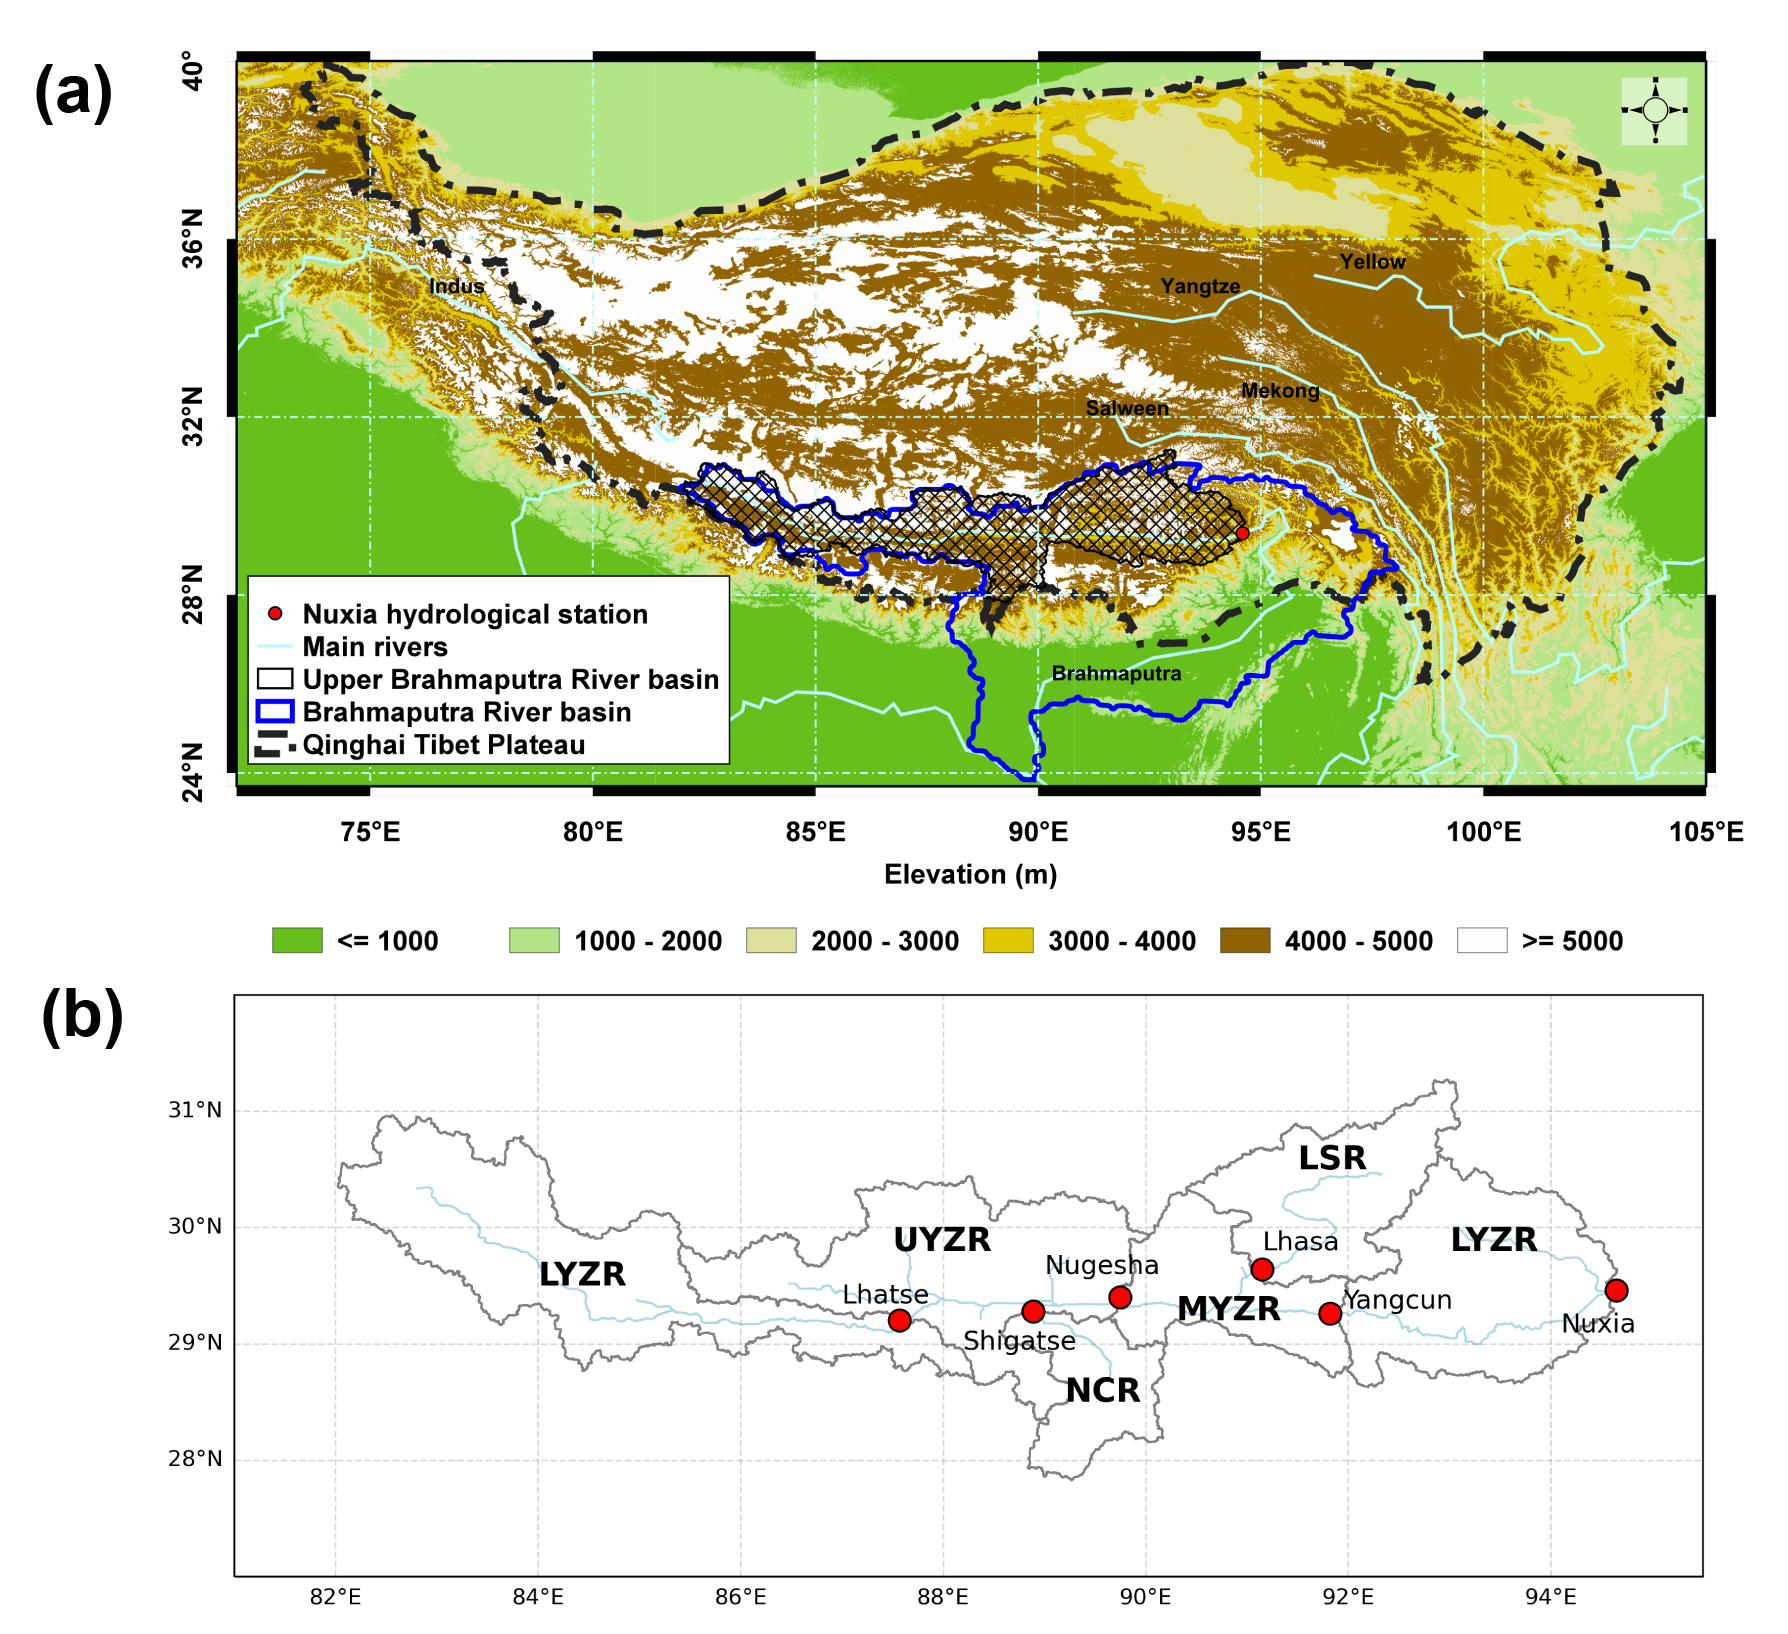
\includegraphics[width=0.8\textwidth]{02-figures/Figure1.png}
    \caption{Location of (a) the Upper Brahmaputra River (UBR) basin in the Qinghai Tibet Plateau (QTP), which is from \citet{li2021vegetation}, and (b) six basins divided by Lhatse, Nugesha, Shigatse, Yangcun, Lhasa, and Nuxia hydrological stations.}
    \label{fig:location}
\end{figure*}

\subsection{Data}
Here, we collect multi-station annual runoff observations from 1982 to 2013 and convert the river flow (m$^{3}$/s) into runoff depth (mm). In addition, we acquire high-resolution climate and vegetation data over the same time period, and further aggregate these gridded datasets into annual values regionally by considering area-weighted effects (their temporal changes are shown in Figure \ref{figS:time series}).

\subsubsection{Runoff data}
Annual runoff observations between 1982 and 2013 used here come from six hydrological stations along the mainstream and major branches in the UBR basin. WY in the HYZR is equal to runoff depth at Lhatse station, while WY in other basins is calculated by the difference between runoff depth from the downstream station and that from the upstream and branch stations. For example, WY in the MYZR basin is equal to the difference between runoff depth in Yangcun station and that in Lhasa and Nugesha stations (Figure \ref{fig:location}b).

\subsubsection{Climate data}
The most recent 10 km gridded daily precipitation data, combining topographic and linear correction approaches based on 262 rain-gauge observations, is developed for the UBR basin by \citet{sun2020precipitation} and here used to estimate regional annual precipitation (P). The maximum 2 m air temperature is obtained from China Meteorological Forcing Dataset \citep{he2020first}. The evaporation (E) with a 0.25$^{\circ}$ spatial resolution is acquired from Global Land Evaporation Amsterdam Model (GLEAM) version 3.5a \citep{martens2017gleam}. GLEAM evaporation has been validated in different biome types in China and showed high correlations with in-situ eddy covariance E \citep{yang2017multi}.

\subsubsection{Vegetation data}
Leaf Area Index (LAI) used in this study is obtained from Global Inventory Monitoring and Modelling System (GIMMS) LAI3g with a spatial resolution of 8 km \citep{zhu2013global}. The product is generated using an artificial neural network trained on the Collection Terra Moderate Resolution Imaging Spectroradiometer (MODIS) LAI product and the latest version of GIMMS NDVI3g data for the same period, which has been proven to have an improved multi-sensor record harmonization scheme compared to other global LAI products \citep{forzieri2020increased,gonsamo2021greening,zhu2016greening}. 

\subsubsection{Land use and cover}
The land use and cover in 2000 with a spatial resolution of 1 km is used to represent the land cover types in the UBR basin. The data is acquired from Resource and Environmental Science Data Center, and is here divided into seven primary land use types, including cultivated land, forestland, grassland, water body, urban land, unused land, and glaciers and snow (Figure \ref{figS:lucc}).

\subsection{Methodology}
\subsubsection{Trend and turning point analysis}
In this study, we use the non-parametric Mann--Kendall test \citep{kendall1938new,mann1945nonparametric} to identify the trend in WY, and Pettitt change detection \citep{pettitt1979non} to identify the turning point (Tp) in WY, where the level of significance is set at 0.05. The Pettitt method has the advantages of being non-parametric, rank-based and distribution-free for finding the turning point in a time series. We then compare the averages of WY before and after Tp to reflect the changes in magnitude, and compare the trends in the two periods to represent the direction changes.

\subsubsection{Double mass curve technique}
The DMC used here is a plot of the cumulative data of one variable versus the cumulative data of another related variable in a concurrent period. It has previously been used to assess the individual effect of climate \citep{gao2011changes}, forest disturbance \citep{wei2010quantifying}, wildfire \citep{hallema2018burned}, and cryosphere \citep{brahney2017determining} on water resources. For the large and pristine UBR and other mountainous basins, climate, vegetation, and cryosphere (melt waters from glaciers and snow under warming, see \citealt{biemans2019importance,huss2018global}) play important roles in the water cycle, and these three components must be considered together to accurately estimate the hydrological response to warming. It is difficult to directly calculate the supply of melt waters to WY due to the lack of long-term glacier monitoring. On the other hand, runoff observations and high-resolution climate and vegetation data make it possible to use the DMC technique, a data-driven statistical method, to estimate cryospheric contributions to WY.  

Appropriate selection of climate and vegetation indices used in the DMC technique is of great importance. Previous studies have shown that effective precipitation (P-E, eP) can adequately represent the impact of climate on WY compared to individual estimates of P or E \citep{wei2010quantifying,zhang2019separating}. LAI quantifies the amount of leaf area in an ecosystem and is an important variable reflecting vegetation structures and biophysical processes \citep{forzieri2020increased}, and \citet{li2021vegetation} has used LAI to investigate vegetation effects on seasonal hydrology in the UBR basin. Hence, we consider eP and LAI as the indices of climate and vegetation respectively, and use their time series as the inputs in the DMC model. 

To obtain cryospheric contributions to WY, we firstly build two types of DMC plots (see Figure \ref{figS:DMC}) to assess the contributions of climate and vegetation, and then subtract the sum of estimated contributions from total WY deviations as cryospheric effects (results are shown in Figure \ref{fig:attribution-results}). The mathematical formulas, relevant descriptions and an example (Figure \ref{fig:example_DMC}) are as follows:

\begin{figure*}[ht]
    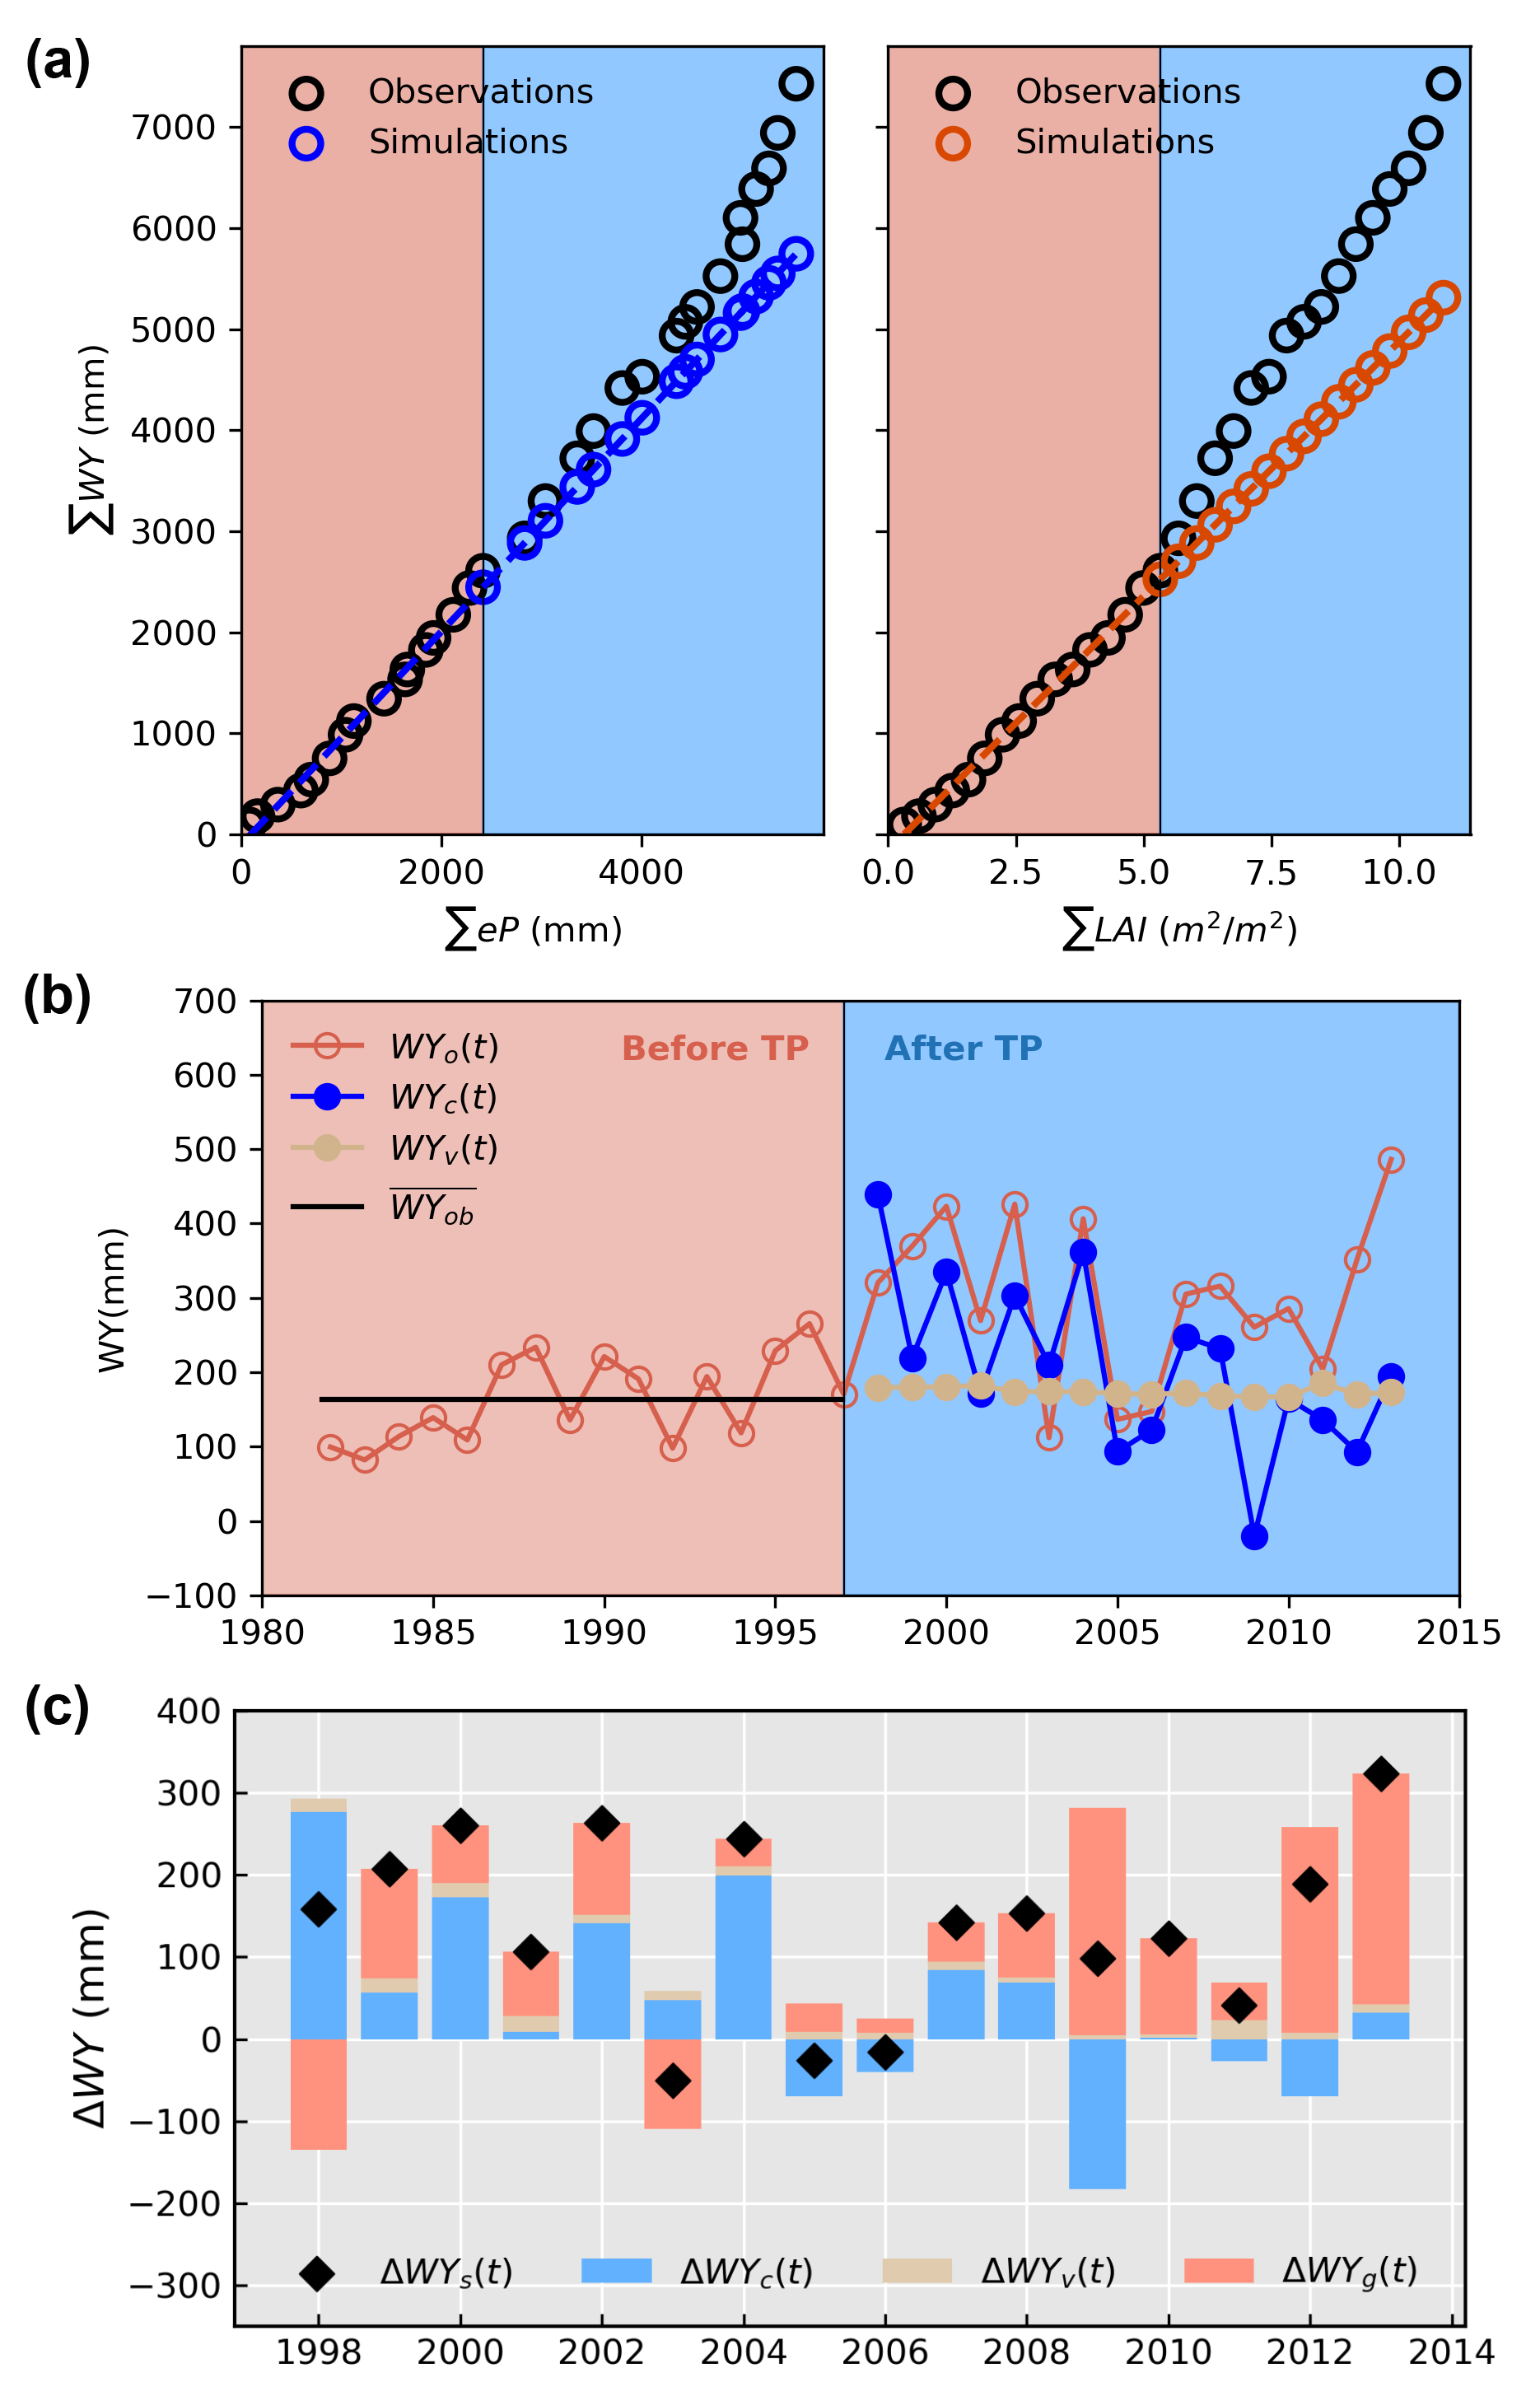
\includegraphics[width=11cm]{02-figures/example_DMC.png}
    \caption
    {The example showing how to estimate the effects of climate, vegetation, and cryosphere on water yield in the MYZR basin (see details in Methodology), where Tp is 1997.}
    \label{fig:example_DMC}
\end{figure*}

First, the average WY before Tp ($\overline{WY_{ob}}$, horizontal black line in Figure \ref{fig:example_DMC}b) is defined as:
\begin{equation}
    \overline{WY_{ob}} = \frac{\sum_{t=1982}^{t=Tp}WY_o(t)} {Tp-1982+1}
\end{equation}

Next, the total WY deviation ($\Delta WY_s(t)$, black diamond in Figure \ref{fig:example_DMC}c) can be calculated as the difference between WY observations after Tp ($WY_o(t)$, red point in Figure \ref{fig:example_DMC}b) and the average WY before Tp ($\overline{WY_{ob}}$), as follows:
\begin{equation} 
    \Delta WY_s(t)=WY_o(t)-\overline{WY_{ob}}, \ \  t=Tp+1, Tp+2, \ldots, 2013
\end{equation}

Second, the regression equation (left panel in Figure \ref{fig:example_DMC}a) between the cumulative eP ($\sum eP$) and cumulative WY ($\sum WY$) before Tp can be constructed as follows:
\begin{equation} \label{eq:2}
    \sum WY = a_1\sum eP + b_1
\end{equation} 

Similarly, the regression equation (right panel in Figure \ref{fig:example_DMC}a) between cumulative LAI ($\sum LAI$) and cumulative water yield ($\sum WY$) before Tp can be constructed as follows:
\begin{equation} \label{eq:3}
    \sum WY = a_2\sum LAI + b_2
\end{equation}

Third, WY driven by climate ($WY_c(t)$, blue line in Figure \ref{fig:example_DMC}b) can be calculated by using the cumulative eP after Tp as input into Equation \ref{eq:2} which is built using the cumulative data of WY and eP before Tp. Therefore, WY deviations caused by climate change ($\Delta WY_c(t)$, blue bar in Figure \ref{fig:example_DMC}c) can be calculated as follows:
\begin{equation}
    \Delta WY_{c}(t)=WY_{c}(t)-\overline{WY_{ob}}, \ \  t=Tp+1, Tp+2, \ldots, 2013
\end{equation}

Similarly, WY driven by vegetation ($WY_v(t)$, tan line in Figure \ref{fig:example_DMC}b) can be calculated via Equation \ref{eq:3}, and WY deviation caused by vegetation ($\Delta WY_v$, tan bar in Figure \ref{fig:example_DMC}c) can be calculated as follows:
\begin{equation}
    \Delta WY_{v}(t)=WY_{v}(t)-\overline{WY_{ob}}, \ \ t=Tp+1, Tp+2, \ldots, 2013
\end{equation}

Finally, WY deviation caused by cryosphere ($\Delta WY_g$, red bar in Figure \ref{fig:example_DMC}c) can be calculated as:
\begin{equation}
    \Delta WY_{g}(t)=\Delta WY_s(t)-\Delta WY_{c}(t)-\Delta WY_{v}(t)
\end{equation}

\subsubsection{Attribution analysis on changes in water yield}
The average contributions of climate, vegetation, and cryosphere to WY magnitude changes are calculated as follows:
\begin{equation}
    \begin{split}
        \overline{\Delta WY_{c}}=\frac{\sum_{t=Tp+1}^{t=2013} \Delta WY_{c}(t)}{2013-Tp}\\
        \overline{\Delta WY_{v}}=\frac{\sum_{t=Tp+1}^{t=2013} \Delta WY_{v}(t)}{2013-Tp}\\
        \overline{\Delta WY_{g}}=\frac{\sum_{t=Tp+1}^{t=2013} \Delta WY_{g}(t)}{2013-Tp}
    \end{split}
\end{equation}

The relative contribution ($RC$), ranging from 0 to 1, of climate, vegetation, and cryosphere can be calculated as follows:
\begin{equation}
    \begin{split}
        RC_{c}=\frac{\left|\overline{\Delta WY_{c}}\right|}{\left|\overline{\Delta WY_{c}}\right|+\left|\overline{\Delta WY_{v}}\right|+\mid \overline{\Delta WY_{g} \mid}}\\
        RC_{v}=\frac{\left|\overline{\Delta WY_{v}}\right|}{\left|\overline{\Delta WY_{c}}\right|+\left|\overline{\Delta WY_{v}}\right|+\mid \overline{\Delta WY_{g} \mid}}\\
        RC_{g}=\frac{\left|\overline{\Delta WY_{g}}\right|}{\left|\overline{\Delta WY_{c}}\right|+\left|\overline{\Delta WY_{v}}\right|+\mid \overline{\Delta WY_{g} \mid}}
    \end{split}
\end{equation}

Additionally, we use the Pearson correlation coefficient ($r$) to quantify the relationships between total WY deviation ($\Delta WY_s(t)$) and its components: WY deviation caused by climate ($\Delta WY_c(t)$), vegetation ($\Delta WY_v(t)$) and cryosphere ($\Delta WY_g(t)$). The Student's t-test with the Bonferroni correction \citep{bonferroni1935calcolo} is used to detect the statistical significance of the correlation coefficient at the level of 0.05.

\section{Results}
\subsection{Long-term changes in historical water yield}
The detection of long-term WY changes in the UBR basin from 1982 to 2013 is illustrated in Figure \ref{fig:water-yield}. There is a high degree of spatial variability in WY (Figure \ref{fig:water-yield}a) across the entire basin. The average WY is the highest in the LYZR basin (over 600 mm), followed by that in the LSR basin (nearly 400 mm). However, the average WY in the HYZR and NCR basins is less than 100 mm. This spatial variability is consistent with that of precipitation (Figure \ref{figS:P-and-WY}), which is mainly determined by elevation and distance to the ocean \citep{sang2016precipitation}. In addition, WY generally increases during the period, as shown by the positive slope in Figure \ref{fig:water-yield}b, even though the significant trend is only detected in the UYZR and MYZR basins (hatched areas in Figure \ref{fig:water-yield}b). Tp mainly occurs during the late 1990s (Figure \ref{fig:water-yield}c), but the abrupt change detected in some basins is not statistically significant (Table \ref{tab:my-table}). Similarly, the cumulative anomaly curve (Figure \ref{fig:water-yield}d) shows that WY decreases prior to the late 1990s and then increases in the entire UBR basin, which further supports the results obtained from the Pettitt method.

\begin{figure*}[ht]
    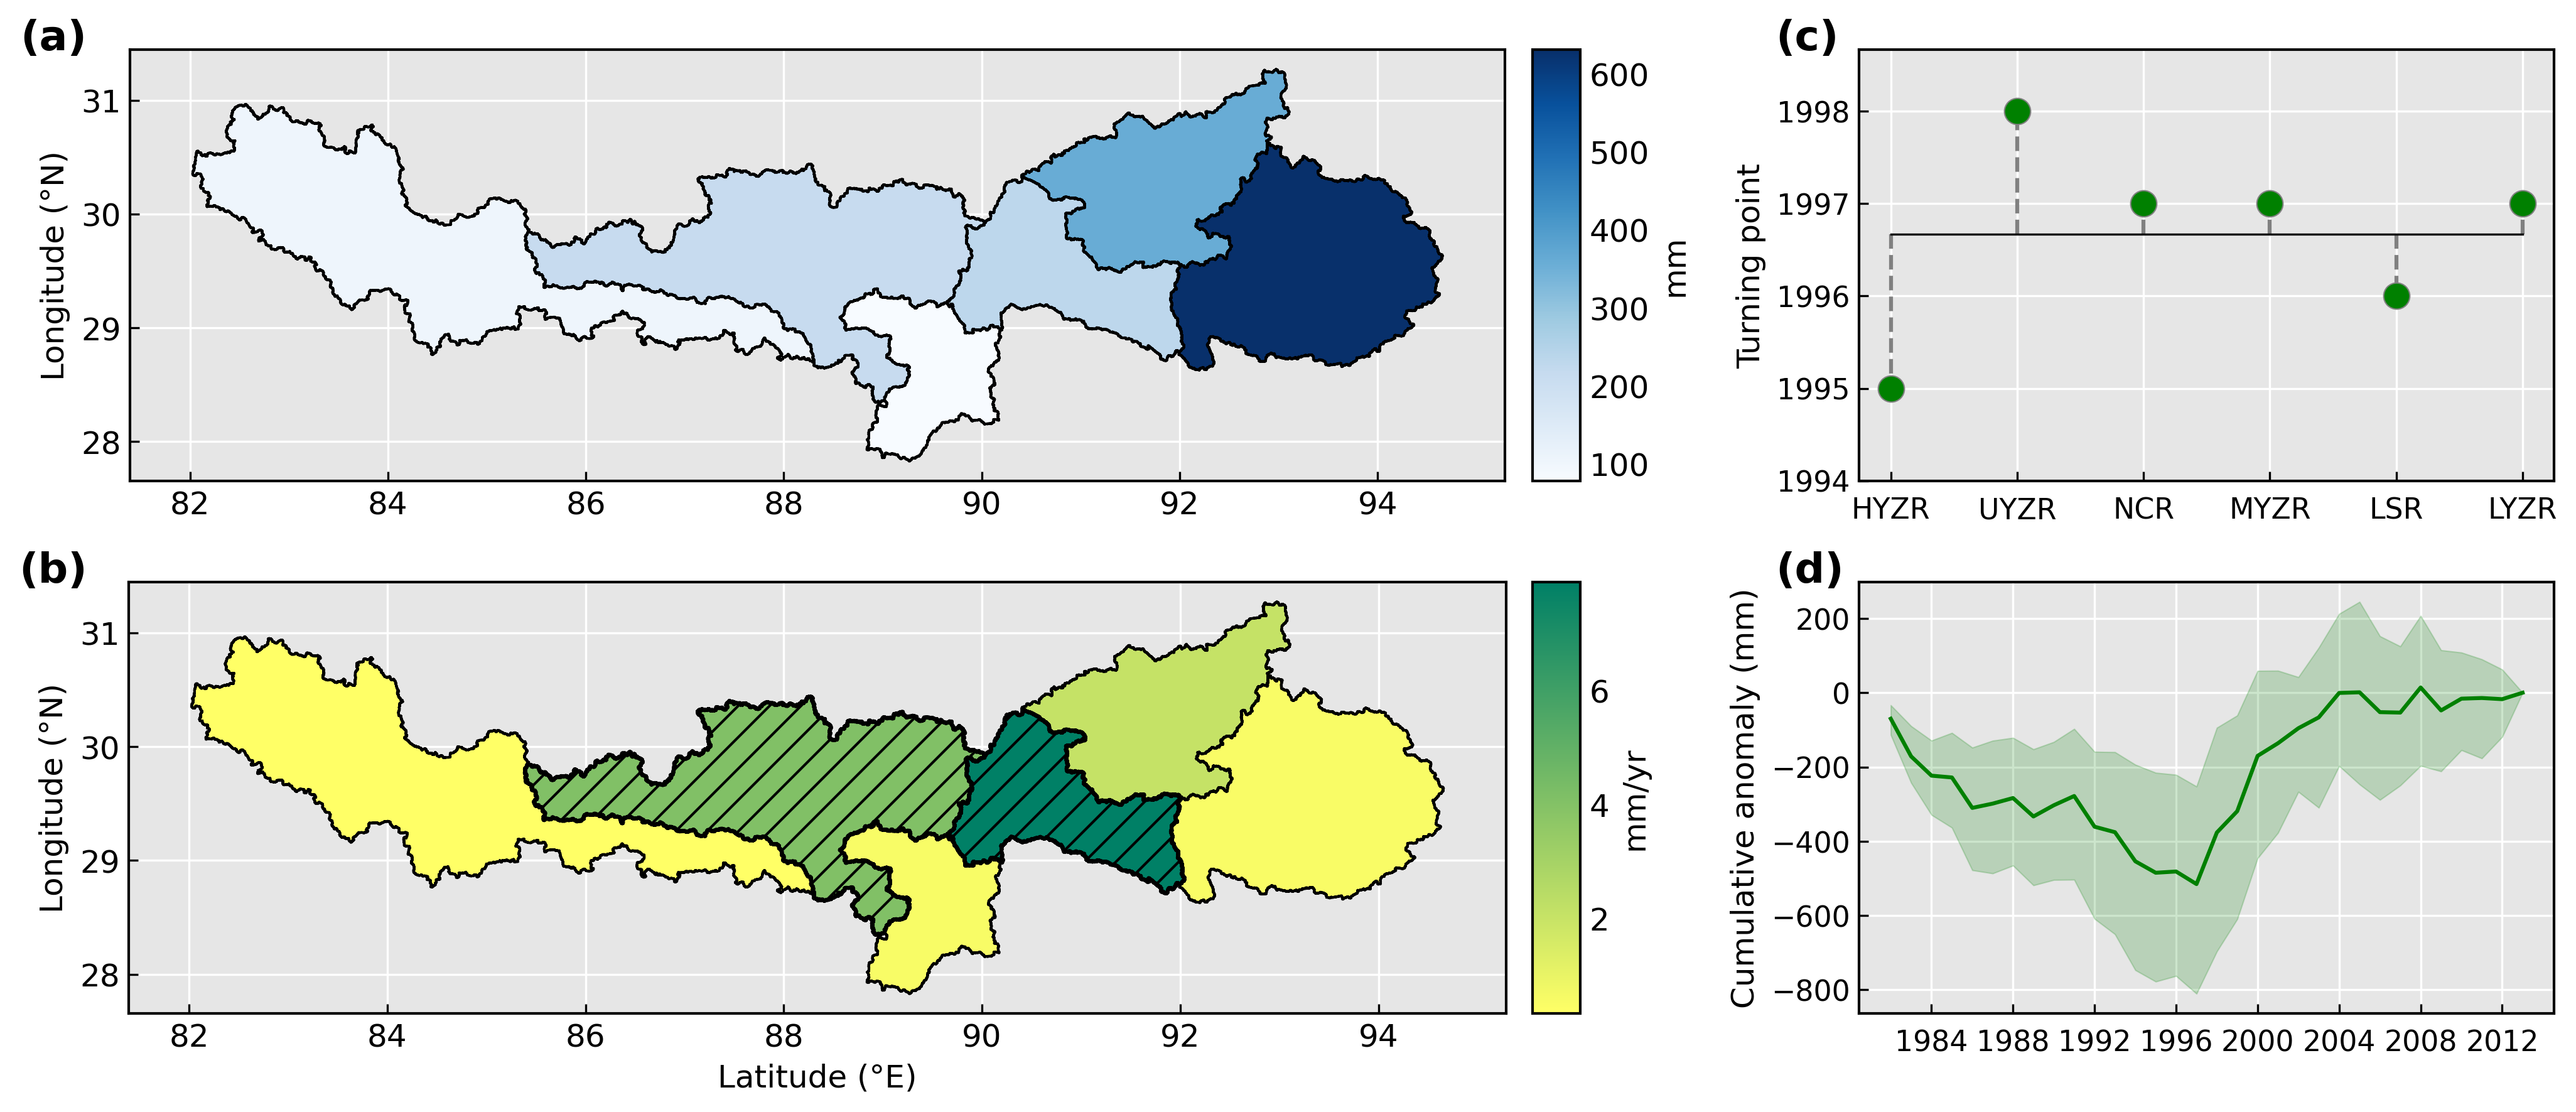
\includegraphics[width=\textwidth]{02-figures/spatial-changes-in-water-yield.png}
    \caption{Long-term water yield changes in the entire UBR basin.
    (a) The annual values calculated by averaging water yield from 1982 to 2013. (b) The temporal trends detected by the Mann-Kendall Sen’s slope method. The black hatching represents statistically significant (p < 0.05) trends. (c) The turning points detected by the Pettitt method. (d) The cumulative anomaly curve of water yield. The solid green line represents the ensemble expectation of cumulative anomaly curves of water yield in the entire UBR basin (green shading).}
    \label{fig:water-yield}
\end{figure*}

\subsection{Regime shifts in historical water yield}
Based on the results of the abrupt detection, we divide the period from 1982 to 2013 into before and after Tp period, and analyze the magnitude and direction of WY changes in the entire UBR basin. Figure \ref{fig:magnitude-direction}a shows that WY increases from 9.5 to 130.9 mm, with a high spatial variability. The slight increase observed in the HYZR and LYZR basins accounts for less than 10\% of the mean WY before Tp, while a substantial WY increase of 61.6\% and 80.5\% is found in the UYZR and MYZR basins, respectively. In addition, higher variability is detected after Tp, suggesting a more dramatic variation in recent years. 
With respect to the direction of change in WY, we find that the trend is positive before Tp, but becomes negative afterward in most basins (Figure \ref{fig:magnitude-direction}b and \ref{figS:time series}). The significantly decreasing trend is detected in the UYZR, NCR, and LSR basins. In contrast, although the WY in the MYZR basin increases during two periods, the rate has slowed; the positive trend after Tp (3.64 mm yr$^{−1}$, p > 0.05) is less than that before Tp (8.95 mm yr$^{−1}$, p < 0.05). Overall, WY regime shifts occur in the late 1990s in the entire UBR basin; the magnitude generally increases, but the direction of WY has reversed or slowed.

\begin{figure*}[ht]
    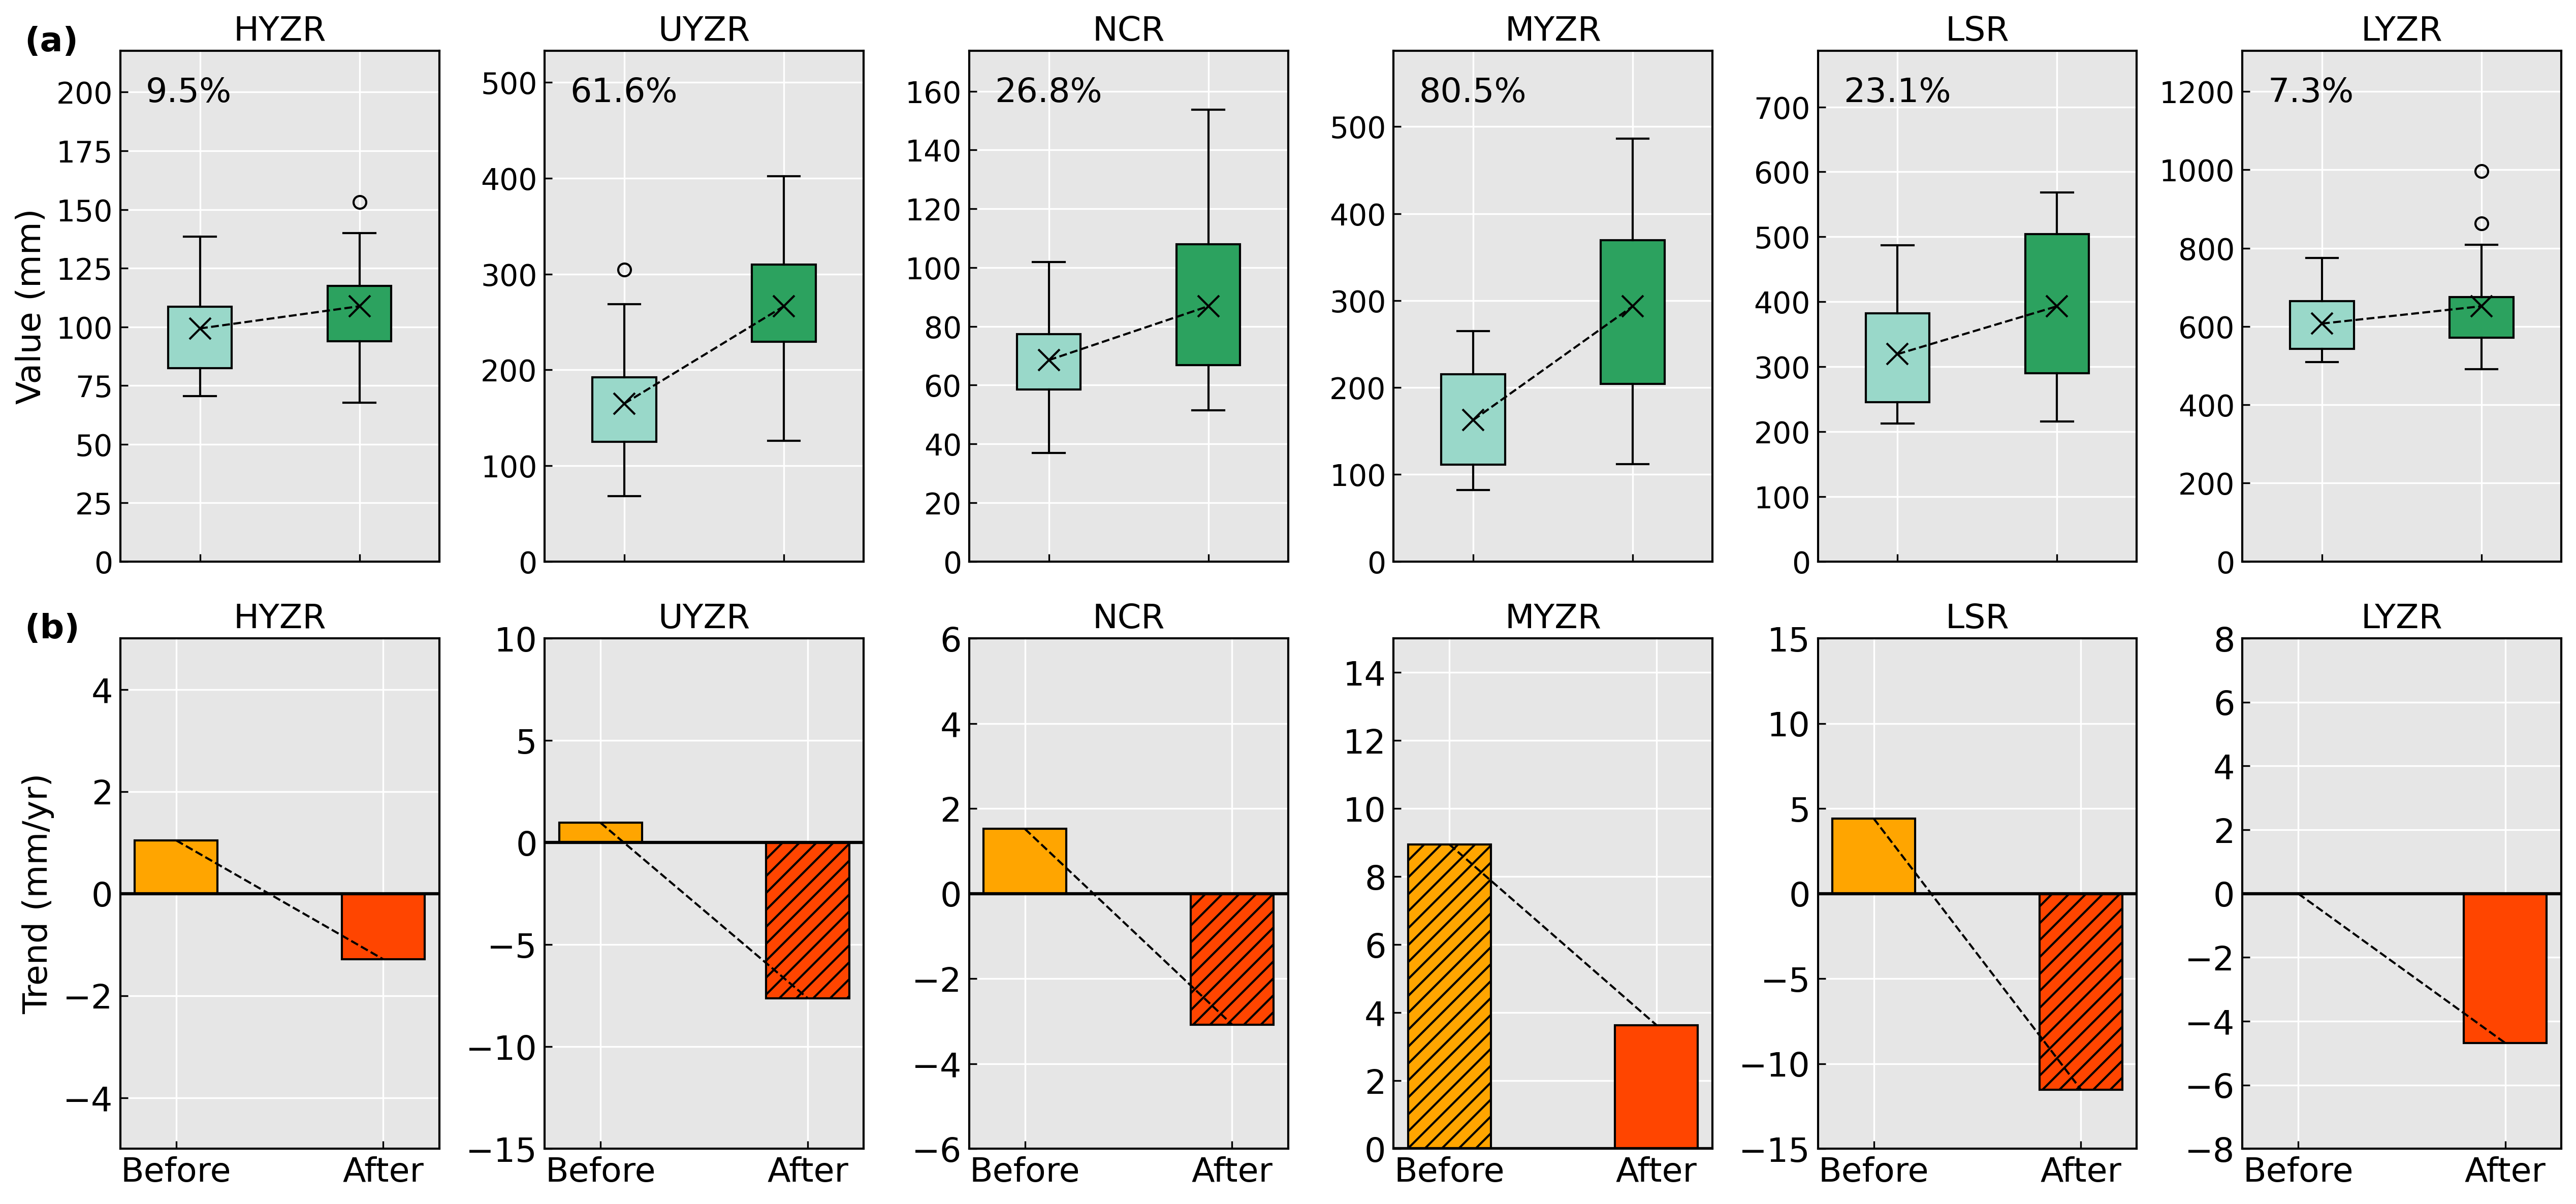
\includegraphics[width=\textwidth]{02-figures/magnitude_and_direction.png}
    \caption
    {Water yield regime shifts in the entire UBR basin. (a) Magnitude of water yield changes. The black "x" signal shows the mean of water yield, and the relative change is labeled in number (\%) in each boxplot. (b) Direction of water yield changes. The black hatching represents the statistically significant trend (p < 0.05). The color of boxes represents before (light color) and after (dark color) Tp period.}
    \label{fig:magnitude-direction}
\end{figure*}

\subsection{Attribution analysis of magnitude increases in water yield}
In Figure \ref{fig:attribution-magnitude}, we quantify the contributions from climate (eP), vegetation (LAI), and cryosphere on WY magnitude increases in the entire UBR basin. We find that cryosphere changes, on average, contribute to over half of WY increases in the HYZR, UYZR, NCR, and MYZR basins. However, climate plays a more important role in WY magnitude increases in the LSR and LYZR basins, with average relative contributions of 55.4\% and 46.0\%, respectively. In contrast to the dominant roles of climate and cryosphere, vegetation has a consistently positive contribution to WY increases, although its relative contribution is much less than those from climate and cryosphere.

Climate and cryosphere -- two important factors affecting WY -- together contribute to over 80\% of the average increases in WY magnitudes over the entire UBR basin. However, they play either additive or offsetting roles in different basins (Figure \ref{fig:attribution-magnitude}) and thus result in slight or substantial WY increases (Figure \ref{fig:magnitude-direction}a). For example, although cryospheric changes contribute to an increase in WY in the HYZR (28.3 mm) and NCR basins (30.3 mm) (black "x" signal in Figure \ref{fig:attribution-magnitude}a+c), the negative contributions from climate offset a considerable part of these increases, leading to only slight increase in WY after Tp in these regions. Similarly, the positive contribution from climate offsets the negative contribution from cryosphere in the LSR and LYZR basins, which also results in a slight WY increase. In addition, the additive effects from climate and cryosphere lead to substantial increases in WY from 162.6 mm to 293.5 mm in the MYZR basin and from 164.9 mm to 266.5 mm in the UYZR basin (Figure \ref{fig:magnitude-direction}a).

\begin{figure*}[ht]
    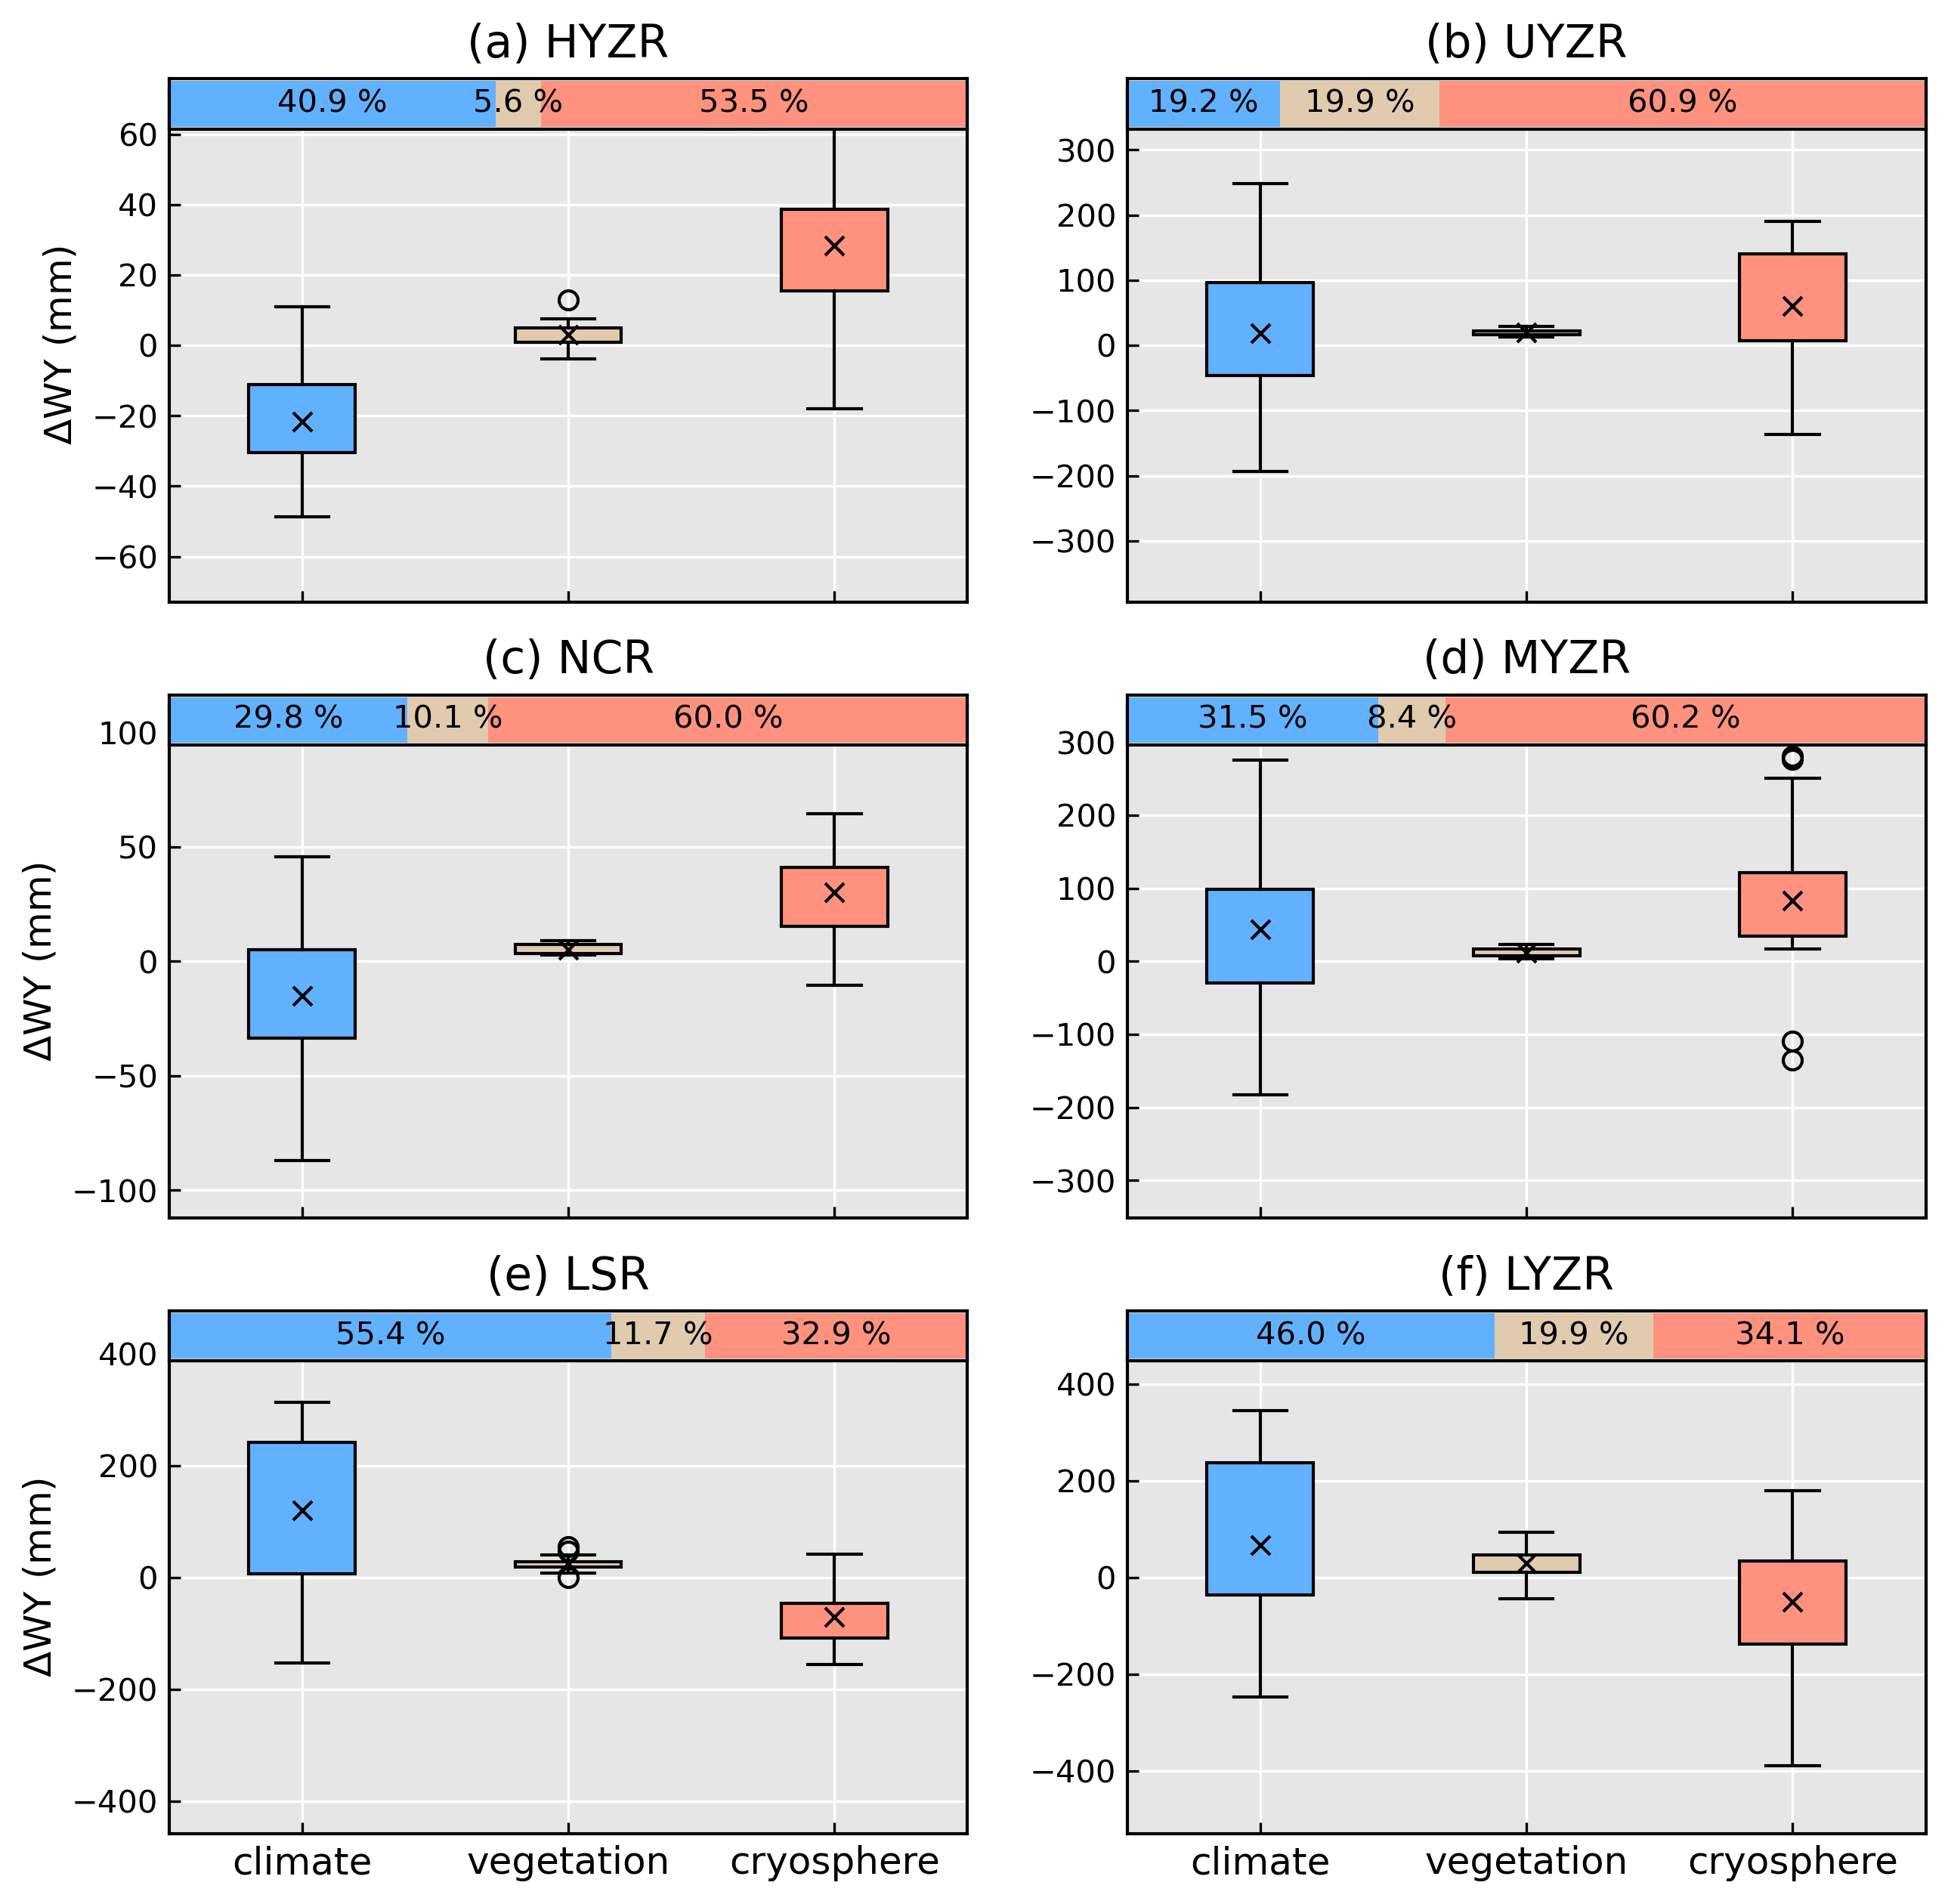
\includegraphics[width=0.8\textwidth]{02-figures/attribution-in-magnitude.png}
    \caption{Attribution analysis of magnitude increases in water yield due to climate ($\Delta WY_c$, blue box), vegetation ($\Delta WY_v$, tan box), and cryosphere ($\Delta WY_g$, red box), and their relative contributions (the bar with colors on the top) in each basin.  The black "x" signal shows the average of water yield deviations (see Figure \ref{fig:attribution-results}) in each boxplot.}
    \label{fig:attribution-magnitude}
\end{figure*}

\subsection{Attribution analysis of direction shifts in water yield}
Pearson correlation coefficient is applied to determine the role of climate, vegetation, and cryosphere in the reversal or slowing of WY trends after Tp, as shown in Figure \ref{fig:magnitude-direction}b. Results in Figure \ref{fig:attribution-direction} show that, although the correlation varies greatly across basins ranging from 0.11 to 0.93 after Tp, climate typically is positively associated with total WY, in which the correlation is significant in half of the basins (p < 0.05), again revealing the major role of climate in influencing the hydrological trends across the entire UBR basin. Further analysis shows that precipitation is much more important because it exhibits a stronger reversal in trend compared with the trend in evaporation (Figure \ref{figS:climate-directions}), which is also similar to directional changes in WY (Figure \ref{fig:magnitude-direction}b). Additionally, despite the weak contribution of vegetation (Figure \ref{fig:attribution-magnitude}), its positive role in WY changes is more apparent in the drier basins (such as the HYZR, UYZR and NCR basins), while the correlation is negative in the relatively humid LYZR basin.

\begin{figure*}[ht]
    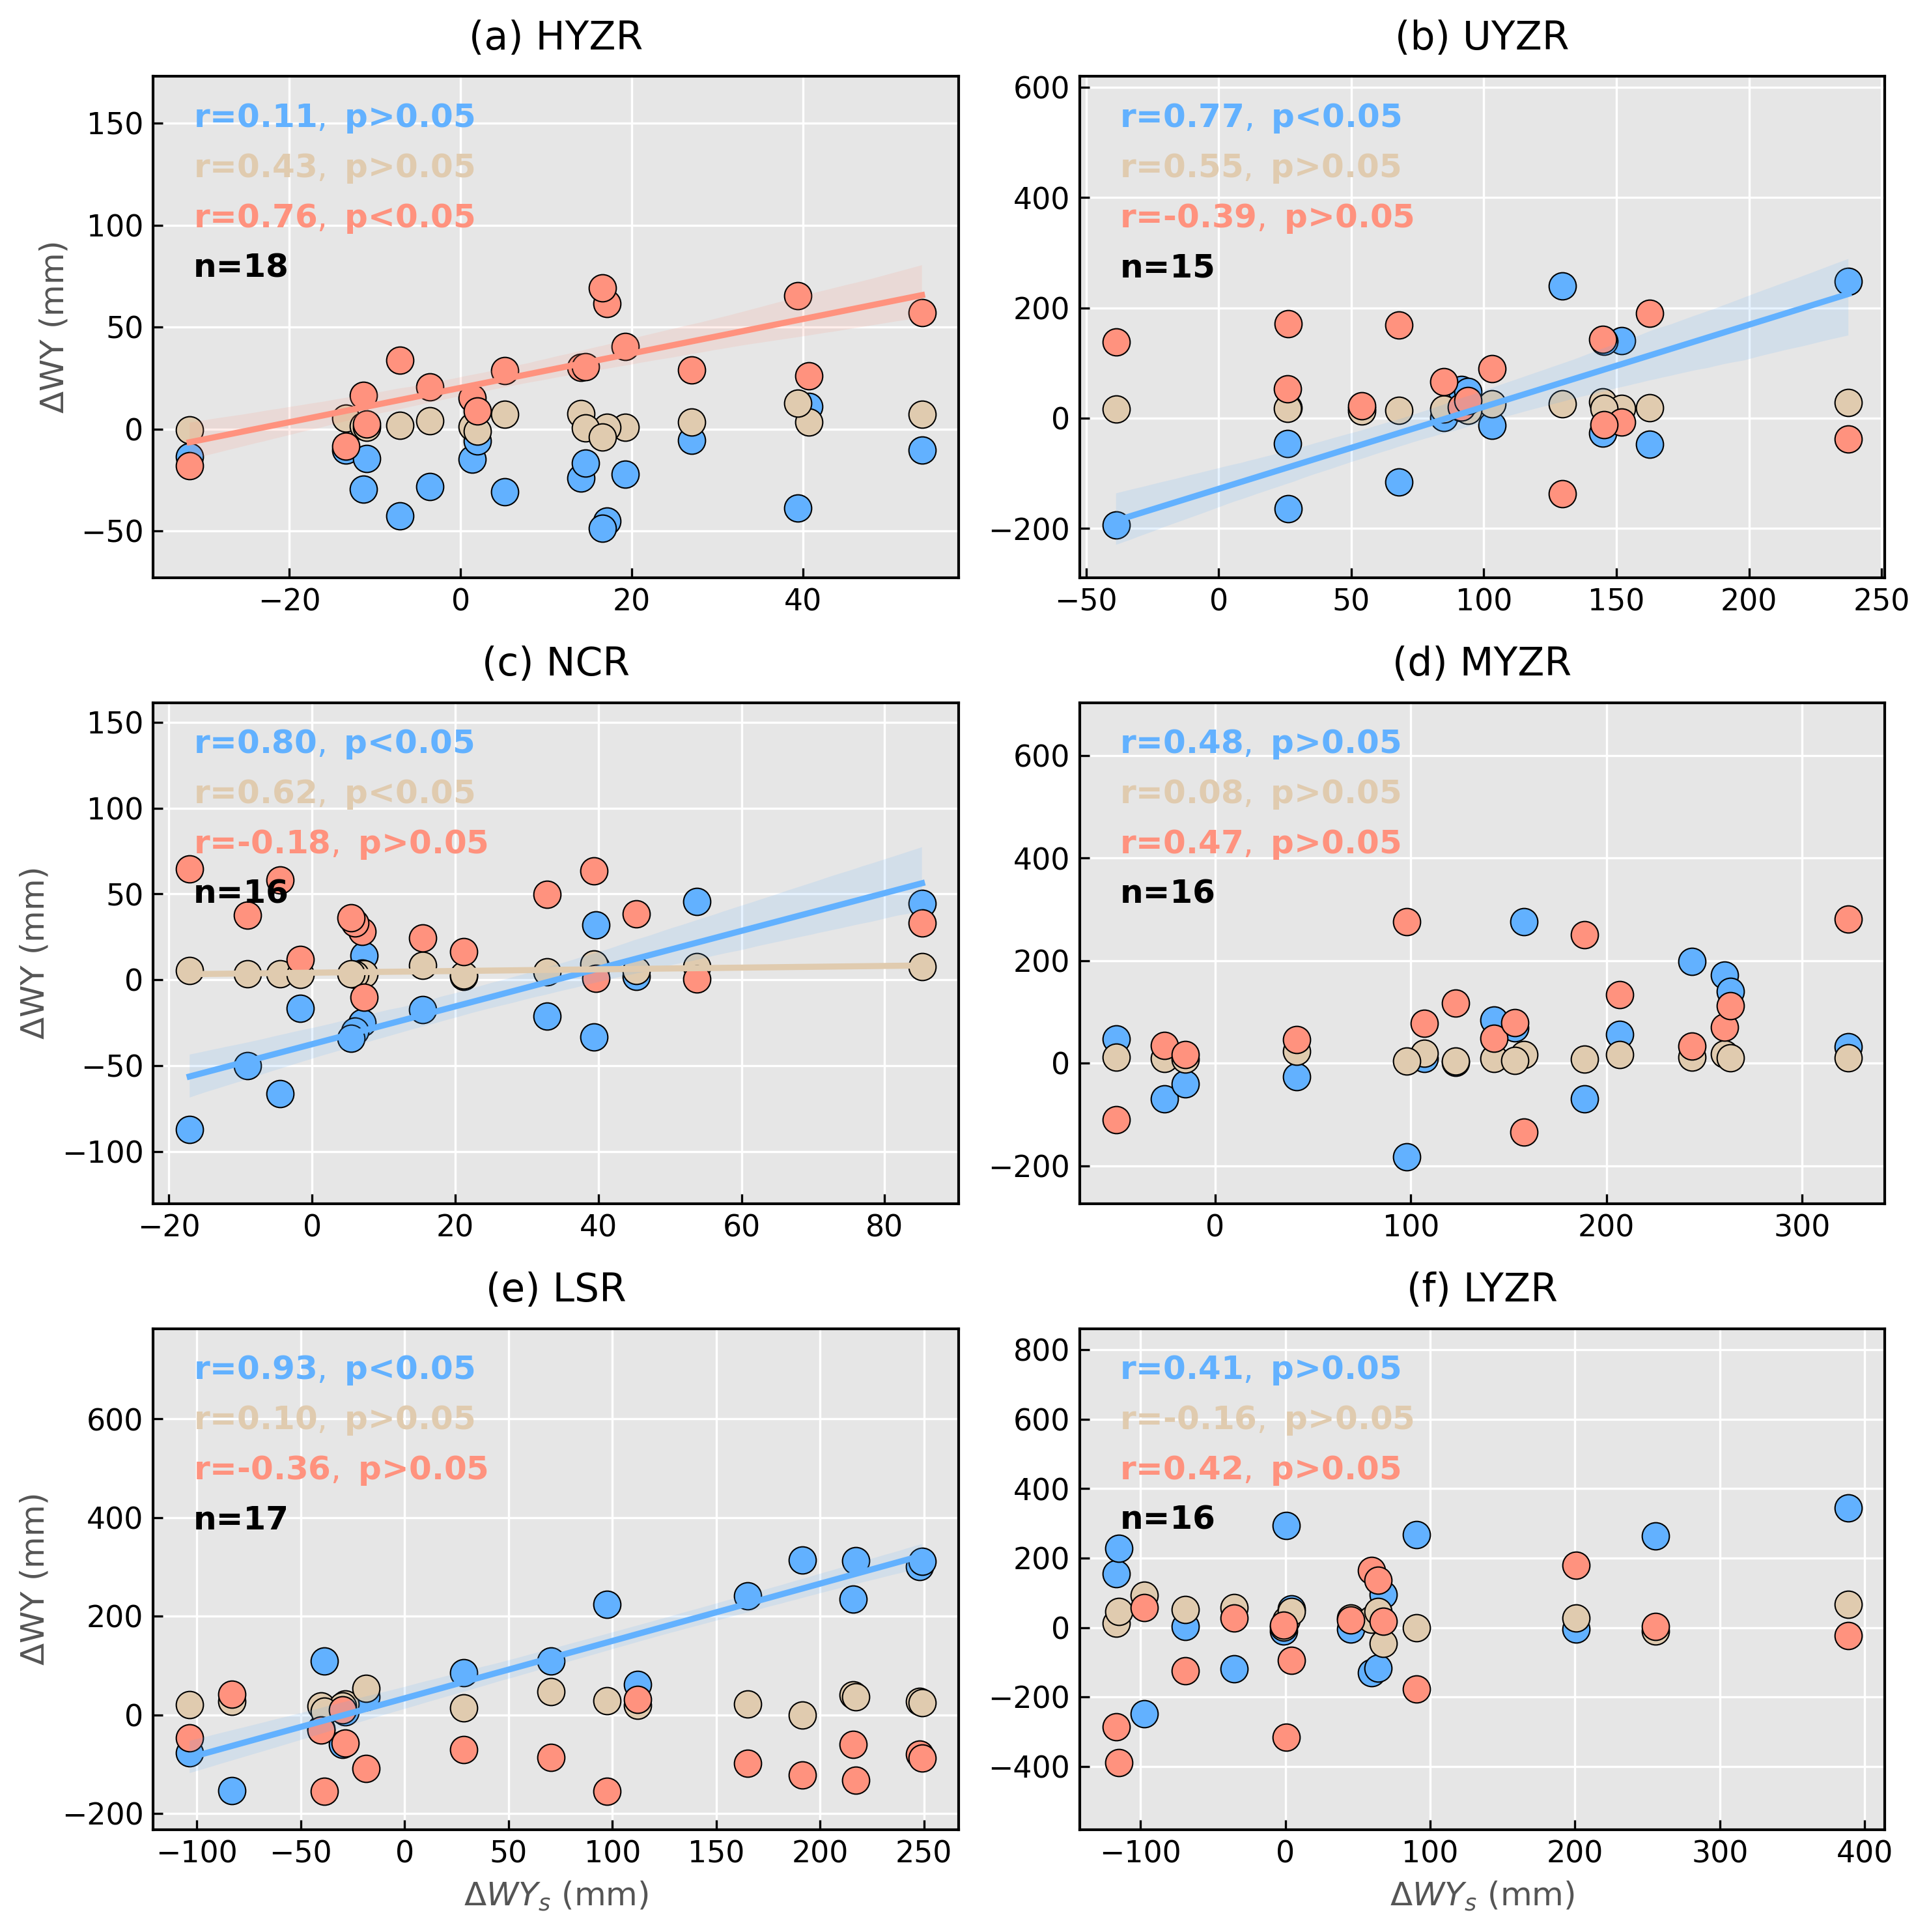
\includegraphics[width=0.8\textwidth]{02-figures/contribution-relations.png}
    \caption{The correlation between time series of total water yield deviation ($\Delta WY_s(t)$, x-axis) and its components (y-axis) caused by climate ($\Delta WY_c(t)$, blue point), vegetation ($\Delta WY_v(t)$, tan point), and cryosphere ($\Delta WY_g(t)$, red point), respectively. The fitting line and its 95\% confidence interval are shown only when p value $<$ 0.05. n indicates the number of years after Tp, which is determined by the Pettitt method (See Table \ref{tab:my-table} and Figure \ref{fig:water-yield}c).}
    \label{fig:attribution-direction}
\end{figure*}

In contrast to positive contributions of climate, we find that WY caused by cryosphere exhibits a negative association with reduced total WY deviations in recent years in the UYZR (r = -0.39, p > 0.05) and LSR (r = -0.36, p > 0.05) basins. The negative but weak relationship indicates that melt waters from cryospheric loss may compensate for low flow, and even mitigate water shortage risks. Also, the compensating effect from cryosphere is stronger in the MYZR (r = 0.47, p > 0.05), and together with climate contributions, contributes to the increasing WY trend (Figure \ref{fig:magnitude-direction}). In contrast to other regions, however, the HYZR basin shows a significantly positive relationship between cryospheric contributions and total WY deviations (r = 0.76, p < 0.05), indicating that the cryosphere instead of climate leads to the downward trend in headwaters. This signifies that in this region, cryospheric contributions may have already passed its potential for supplying to river flow, due to decreased glaciers and snow under continuous warming. This is further verified by the relationship of cryospheric contributions to total WY ($RC_g$) with temperature (Figure \ref{figS:warming-and-cryosphere}a); cryospheric contribution to WY increases with temperature in the beginning until a maximum is reached, and then begins to decrease. In addition, the compensating effect of melt waters can be seen in the UYZR, MYZR and LSR basins, i.e., WY caused by cryospheric changes keeps a positive relationship with the increase in temperature, further supporting the observed higher correlation in these basins (Figure \ref{fig:attribution-direction}).

\section{Discussion}

\subsection{Climate and cryosphere cause water yield regime shifts}
Previous studies have reported the increasing WY trend in the LSR \citep{linhess2020}, LYZR \citep{zhangech2011}, and UBR basin \citep{li2021vegetation}. Here, we not only provide further evidence on the long-term trend of WY changes in the above regions, but also conduct trend analyses in other regions that have received less attention. As such, the study comprehensively indicates a general increase in WY (Figure \ref{fig:water-yield}a) in the entire UBR basin. Further, we find that regime shifts of WY occur during the late 1990s in the entire UBR basin -- the magnitude in WY increases (Figure \ref{fig:magnitude-direction}a), but the direction has reversed or slowed after Tp (Figure \ref{fig:magnitude-direction}b). The result agrees with climate shifts (Figure \ref{figS:time series}), drought changes \citep{li2019spatiotemporal}, and lake area changes \citep{zhang2017} in this region.

Attribution analysis of WY magnitude shifts highlights the dependency of spatial gradients of climate and cryosphere accounting for WY changes. Climate explains a greater increase in WY in downstream regions, while melt water is more important in upstream regions (Figure \ref{fig:attribution-magnitude}). 
This may be attributed to divergent water supply sources; \citet{biemans2019importance} indicates that melt waters supply over 40\% of river flow in the upper regions, but the contribution is less than 30\% in the downstream regions of the UBR basin (Figure \ref{figS:Biemans}). Vegetation does not significantly affect total river flow in the UBR (Figure \ref{fig:attribution-magnitude}), despite its remarkable role in seasonal runoff detected by \citet{li2021vegetation}. 

Climate, especially precipitation, still controls the declining WY trend after Tp in most regions (Figure \ref{fig:attribution-direction} and \ref{figS:climate-directions}), and may become an important factor in occurrence of turning points (Figure \ref{fig:water-yield}c+d). This suggests the importance of precipitation and its projections on future hydrological process in mountainous watersheds \citep{lutz2014consistent}. Cryospheric contribution is also important for water yield regime shifts -- melt waters from glaciers and snow can alleviate water resources shortages, mainly caused by decreased precipitation in recent years (Figure \ref{fig:attribution-direction} and \ref{figS:climate-directions}). This finding is also supported by observed glacier runoff data \citep{yao2010glacial} and several modeling studies \citep{lutz2014consistent, Zhang2020VariationOM, wang2021tp}. However, after glacier runoff reaches a maximum (defined as "peak water" \citep{gleick2010peak}), cryospheric mass loss cannot sustain the rising melt waters with atmospheric warming (e.g. the HYZR basin in Figure \ref{figS:warming-and-cryosphere}), which is in agreement with \citet{huss2018global}. 

\subsection{Uncertainties and limitations}
%%%%%%%%% Method Limitations 
This study has some limitations pertaining to the DMC model used for partitioning the effects of climatic and cryospheric changes on the hydrological regime shifts in the UBR basin. The DMC method is a useful statistical alternative to physical modeling approaches, especially in alpine river basins (e.g. UBR basin) where there is inadequate knowledge of the complex hydrological mechanisms. However, the method is still dependent on our prior understanding of hydrological responses to warming and related environmental changes, such as glaciers melting and vegetation changes. For the UBR basin, besides climate change, cryosphere \citep{biemans2019importance,yao2019recent} and vegetation \citep{li2021vegetation,li2019greening} are two major factors which drive hydrological changes. Here, the cryospheric contribution is estimated as the deviation between total water yield and the climate and vegetation contribution estimated by the DMC method. However, in some mountainous basins, human activities such as urbanization, dam regulation and irrigation may consume a significant portion of water resources or induce changes in seasonal runoff patterns. Therefore, it is necessary to account for anthropogenic impacts when assessing river flow changes via the statistical models in these regions, in addition to the factors considered in this study. In addition, the DMC method assumes a linear relationship between two variables, and thus it may fail to capture nonlinear interactions among water, vegetation and cryospheric melting. For example, the role of vegetation in influencing hydrological responses is expected to be complex due to biophysical (e.g., via transpiration and albedo changes) and biochemical (e.g., via CO2 uptake and release) feedbacks (\citealt{bonan2008forests,krich2022decoupling,li2021vegetation}). Thus, with the availability of long-term in-situ observations and high-resolution remote sensing datasets in the UBR basin \citep{wang2022observing}, other powerful statistical models which account for nonlinear and casual relationships should be applied to identify the causes of water yield changes \citep{runge2019inferring}.

%%%%%%%%% Data Limitations 
The data used in the study is another source of uncertainty in our results. The precipitation dataset used here is generated by topographical and linear corrections based on observations. As \citet{sun2020precipitation} have pointed out, the results of the linear correction approach vary significantly with station density. For example, increasing the number of stations from 4 to 10 in the basin results in a decrease of the mean annual precipitation estimate by about 20 mm. Hence, the reconstruction of the precipitation dataset will rely on the density of the observed stations. Besides the topographic correction, the effects of basin size and climate seasonality should be considered in the work of precipitation reconstruction in the UBR basin due to its complex climate and environment \citep{sun2019contrasting}. Compared with precipitation, the estimation of evaporation may be much more challenging in high mountains. Although GLEAM evaporation shows good agreement with in-situ eddy covariance records \citep{yang2017multi}, its model structure does not include wind speed and solar radiation, which may affect the estimation of sublimation, and thus total evaporation \citep{li2019evapotranspiration}. 
In addition, the coarse spatial resolution (0.25$^{\circ}$) of GLEAM may be insufficient to estimate regional evaporation in the UBR basin.
GIMMS LAI has the advantage of capturing ecosystem structure, and thus is widely used to assess vegetation conditions and their effects on hydrological changes \citep{zhu2016greening,forzieri2020increased,gonsamo2021greening}. However, LAI ignores the vegetation's physiological process \citep{fang2019overview}. \citet{hu2022decoupling} have indicated that LAI can cope with hydro-climatic fluctuations in arid environments, but the tradeoff between ecosystem structure (LAI) and physiology (photosynthesis per unit leaf area) is stronger in humid climates. Thus, using LAI products in energy-limited regions may result in some biased assessments of vegetation effects on water yield.
Inspite of the uncertainties in the methods and data used here, this study provides essential information for water resource management in the UBR basin based on multi-station runoff observations. With the help of the Second Tibetan Plateau Scientific Expedition and Research, the observation networks in meteorology, cryosphere, and hydrology will be expanded, which can potentially lead to better understanding of the hydrological processes in this region, and make developing physically-based cryosphere-hydrological modeling possible \citep{wang2022observing}.

\subsection{Broad Implications for mountainous water management}
Understanding the hydrological regime shifts and their causes in high mountain regions is especially important in managing water resources. Of specific importance is balancing the co-benefits between mountains and downstream lowlands \citep{viviroli2011climate}. In this study, the combined (both offsetting and additive) effects of climate and cryosphere are detected (Figure \ref{fig:attribution-magnitude}). They further lead to either slight or substantial increases in WY across the entire UBR basin (Figure \ref{fig:magnitude-direction}a). The combined effects often hinder the role of each driver in influencing hydrological changes \citep{wei2018,zhang2021deforestation}, and thus should be considered when designing water management strategies in large transboundary river systems. For example, the additive effect may be beneficial for mitigating droughts and water shortage during droughts, but it may exacerbate flood risks due to increased precipitation and accelerated melting of the cryosphere in the future \citep{Immerzeel2013}. In addition, in the headwaters, WY resulting from cryosphere melting continues to increase with temperature until a maximum is reached, beyond which cryospheric contribution to total WY begins to decrease (Figure \ref{figS:warming-and-cryosphere}a). This shows that the melt waters from glaciers may have already surpassed the "peak water" time. Such hydrological changes will substantially affect future water resources management, and thus accurate projections of the occurrence time of "peak water" will be important in managing mountainous water resources.

\conclusions 
In this study, regime shifts in historical WY are detected during the late 1990s in the UBR basin. The WY magnitude generally increases, but its direction has reversed or slowed in recent years. Attribution analysis based on the DMC method shows that the combined effects of climate and cryosphere are either offsetting or additive, leading to slight or substantial WY increases, while the role of vegetation is much weaker. The declining or slowing WY trend after Tp is mainly driven by precipitation in most regions, while melt waters may alleviate drought and water shortage. In headwaters, however, cryospheric contributions to WY have declined due to reduced glaciers under warming. These findings suggest that the combined effects of climate and cryosphere should be considered in the sustainable development of water resources, especially involving co-benefits in upstream and downstream regions.

\codeavailability{Python scripts used to extract data, analyze data, and create figures are available via \url{https://github.ugent.be/haohaoli/HESS-2022-Water-Yield.git}.}

\dataavailability{Annual runoff data during 1982 and 2013 from six hydrological stations are provided by the Hydrology and Water Resources Survey Bureau of the Tibet Autonomous Region. The 10 km gridded daily precipitation dataset is accessed throughout \url{https://www.tpdc.ac.cn/}. The GLEAM evaporation is accessed from \url{https://www.gleam.eu/}. The maximum 2 m air temperature is acquired via \url{https://www.tpdc.ac.cn/}. The map of land use types in 2000 is accessed from \url{https://www.resdc.cn/}.} 

\authorcontribution{H.L. led the effort to design, conduct, analyze and write this manuscript. Other authors analyzed and commented on the results.} %% this section is mandatory
%HL: conceptualisation, data curation, formal analysis, methodology, writing--original draft, writing -- review and editing. LL: conceptualisation, formal analysis, methodology, writing -- review and editing, funding acquisition. BYS: data curation, methodology. LW: supervision, writing -- review and editing. AK: validation, writing -- review and editing. FZ\&DFL: software, validation. XXW: visualization. WFL\&XPL: Writing -- review \& editing. ZXX: supervision, resources.

\competinginterests{All authors have declared that neither they have any competing interests.} %% this section is mandatory even if you declare that no competing interests are present

%\disclaimer{TEXT} %% optional section

\begin{acknowledgements}
    This work is jointly supported by the China Scholarship Council (Grant No. 202006350051), the National Natural Science Foundation of China (Grant No. 51961145104, 52079138, and 91647202), and the 2115 Talent Development Program of China Agricultural University (00109019). H.L. thanks the China Scholarship Council for providing financial support to pursue his PhD in Belgium. We thank Dr. Florian Ulrich Jehn and two anonymous reviewers for their contribution to the peer review of this work.
\end{acknowledgements}


%% REFERENCES
\bibliographystyle{copernicus}
\bibliography{reference.bib}

%\sampleavailability{TEXT} %% use this section when having geoscientific samples available

%\videosupplement{TEXT} %% use this section when having video supplements available

%\noappendix       %% use this to mark the end of the appendix section. Otherwise the figures might be numbered incorrectly (e.g. 10 instead of 1).
%\appendix
%\section{}    %% Appendix A

%\subsection{}     %% Appendix A1, A2, etc.

%% Regarding figures and tables in appendices, the following two options are possible depending on your general handling of figures and tables in the manuscript environment:

%% Option 1: If you sorted all figures and tables into the sections of the text, please also sort the appendix figures and appendix tables into the respective appendix sections.
%% They will be correctly named automatically.

%% Option 2: If you put all figures after the reference list, please insert appendix tables and figures after the normal tables and figures.
%% To rename them correctly to A1, A2, etc., please add the following commands in front of them:

%\appendixfigures  %% needs to be added in front of appendix figures
%\appendixtables   %% needs to be added in front of appendix tables
%% Please add \clearpage between each table and/or figure. Further guidelines on figures and tables can be found below.

\end{document}
